\documentclass[a4paper]{article}

\usepackage[spanish]{babel}
\usepackage[utf8]{inputenc}
\usepackage{amsmath}
\usepackage{graphicx}
\usepackage{tikz}
\usetikzlibrary{shapes,arrows}
\usepackage[colorinlistoftodos]{todonotes}
\usepackage{booktabs}
\usepackage{graphicx}
\usepackage[onehalfspacing]{setspace}

\title{Rastreo de objetos utilizando SURF: Una implementación en paralelo}

\author{Ricardo Antonio Ocampo Vega}

\date{\today}

\begin{document}
\maketitle


\begin{abstract}
El análsis en tiempo real de imágenes y video es importante ya que existen en el mercado dispositivos que pueden aprovechar las bondades del análisis en todo momento de datos. Aunque este interés se ha hecho presente desde hace decadas, no se ha prestado mucha antención en el avance en el desarrollo de algoritmos paralelos. En el presente reporte se muestra el beneficio que se puede obtener al paralelizar un algoritmo. En este caso se paraleliza un algoritmo para rastreo de objetos. En el análisis se llega a obtener un SpeedUp de hasta 4.66x, lo que permite que se reastreen objetos en tiempo real para imágenes de resolución 1280x760.
\end{abstract}

\section{Introducción}
El análisis en tiempo real de imágenes y video es utilizado en distintos sectores. El aspecto de tiempo real es crítico para muchos dispositivos o productos como teléfonos móviles, cámaras, televisiones, sistemas de vigilancia, dispositivos de imágenes médicas, entre otras.

Aunque la investigación detrás del rastreo de objectos ha estado presente durante décadas, la documentación del algoritmos paralelos es escasa.  

Algunas de las aplicaciones del rastreo de objetos son: (1) reconocimiento de rostros humanos \cite{5374808}, control visual \cite{6417913}, segmentación de objetos \cite{6466854}, localización de vehículos \cite{6469511}, entre otras aplicaciones.

La metodología que se utiliza en este caso está compuesta por los siguientes pasos: 
\begin{enumerate}
   \item \textbf{Localización de puntos clave:} Se buscan los pixeles que mejor representan el objeto que se quiere rastrear.
   \item \textbf{Cálculo de los descriptores:} Para cada punto clave, se calcula un vector con característicos. Estos característicos van desde 16 hasta 128 enteros que permiten diferenciar cada uno de los puntos.
   \item \textbf{Empate de puntos similares:} Los puntos cuya distancia euclideana no sobrepase un límite, son apareados.
   \item \textbf{Homografía:} Para los puntos claves que se obtienen, se calcula la matriz de homografía. 
   \item \textbf{Transformación de perspectiva:} Se transforman los puntos que rodean el objeto encontrado y se ajustan a la perspectiva actual.
\end{enumerate}

Los pasos de la metodología, anteriormente mecionados, son algoritmos complejos. Al ser programados secuencialmente, no es posible analizar en tiempo real las imágenes con una resolución mayor a 640x480. 

\subsection{Objetivos}
En el presente documento se reporta la implementación de un método de rastreo de objetos de forma paralela. El objetivo principal es: programar un método en paralelo para el rastreo de objetos que posibilite el análisis de video de manera fluida en tiempo real. Algunos de los objetivos específicos son:

\begin{itemize}
	\item Verificar el speedup obtenido en comparación con el algoritmo secuencial.
    \item Verificar el aumento de frames por segundo entre la implementación secuencial y la implementación en paralelo.
\end{itemize}

\subsection{Alcance}
En este reporte se busca paralelizar ciclos \emph{for} y algoritmos que ya son implementados en librerías como openCV. En caso en que el algoritmo complejos que no estén programado previamente se mantendrán de secuenciales. 

\section{Conocimientos previos}
En esta sección se hace una introducción a los conceptos básicos necesarios para entender la metodología.

\subsection{Detección de atributos invariantes}
El objetivo principal de la detección de atributos invariantes es convertir una imagen en un conjunto de pixeles clave con atributos que los permitan distinguirse entre ellos. Es importante que los atributos sean invariantes a traslación, escala, rotación, cambios de iluminación y distorsión geométrica. No obstante, pocos de los algoritmos cumplen las restricciones anteriores. 

Lowe \cite{lowe2004distinctive} fue el pionero en la detección de pixeles clave y sus descriptores. Aunque es un algoritmo que es preciso, su uso no está abierto al público en general ya que está patentado. Una alternativa, y el algoritmo que se utiliza en nuestra metodología es SURF. SURF es un algoritmo propuesto por Bay \cite{bay2006surf} el cual es un algoritmo de detección de pixeles clave y descriptivos que es mejor que SIFT con respecto a la repetibilidad, es más robusto y más rápido \cite{bay2006surf}. Aunque el aspecto más importante de SURF es que tiene una licencia no comercial. Existen algunas alternativas como FAST \cite{trajkovic1998fast}, ORB \cite{rublee2011orb}, BRISK \cite{leutenegger2011brisk}, y FREAK \cite{alahi2012freak}; aunque en los experimentos realizados estos algoritmos no se desempeñaron mejor que FAST y SURF.

\subsection{Emparejamiento de atributos}
En el emparejamiento de atributos se busca encontrar parejas de pixeles clave que tengan una alta probabilidad de que el pixel del objeto y el pixel de la escena sean el mismo. En la Figura 1, se muestra como se emparejan los pixeles clave del objeto (imagen de la izquierda) con los pixeles clave de la escena (imagen de la derecha). Para el emparejamiento de atributos se utiliza un emparejador de fuerza bruta \cite{muja2009fast, muja2012fast, muja2014scalable}, la cual es una librería para realizar aproximaciones rápidas de búsquedas de vecinos cercanos en espacios de grandes dimensiones. Selecciona de forma automática el mejor algoritmo y parámetros óptimos dependiendo la base de datos. 

\begin{figure}
  \centering
  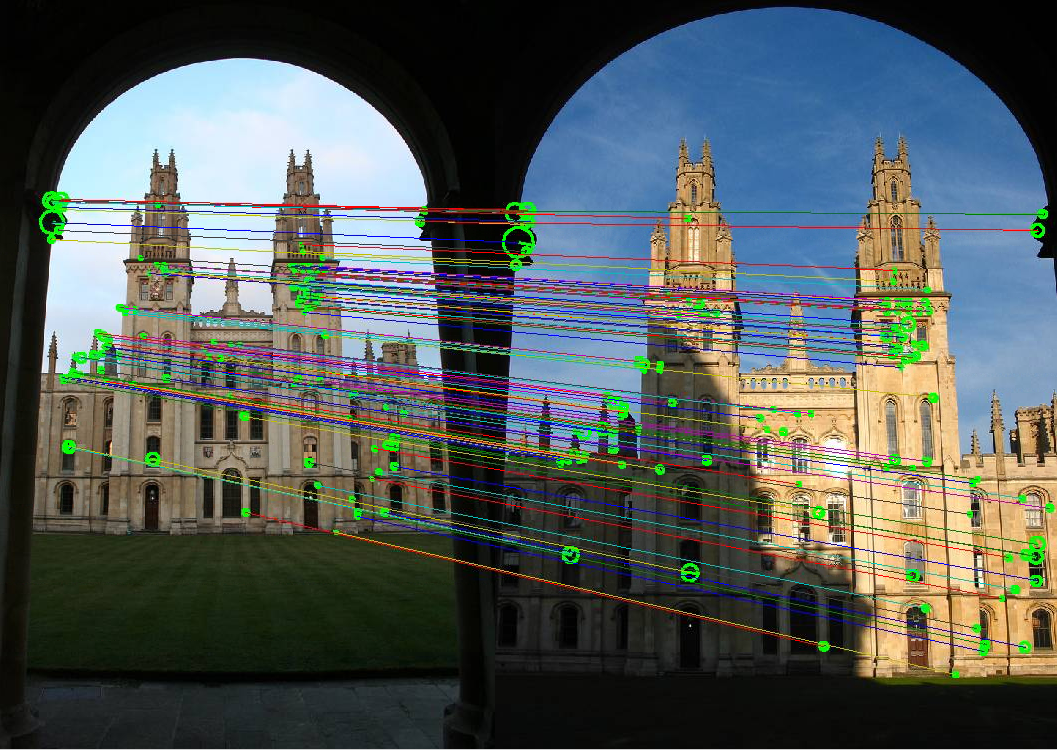
\includegraphics[width=\textwidth]{matching}
  \caption{Figura donde se ilustra como se hace el emparejamiento de pixeles clave entre un objeto y la escena.}
\end{figure}

\section{Metodología}
En la sección anterior se describen brevemente los conceptos necesarios para entender la metodología. En esta sección se describe paso paso la metodología.

\subsection{Descripción del algoritmo}
En la Figura \ref{fig2}, se presenta el diagrama de flujo que se sigue para el rastreo de un objeto en tiempo real. En las subsecciones siguientes se describe paso a paso cada uno de los procesos.

\begin{figure}
  \tikzstyle{decision} = [diamond, draw, fill=blue!50, 
      text width=7em, text badly centered, node distance=3cm, inner sep=0pt]
  \tikzstyle{block} = [rectangle, draw, fill=blue!20, 
      text width=8.5em, text centered, rounded corners, minimum height=2em]
  \tikzstyle{line} = [draw, -latex', -triangle 90]
  \tikzstyle{cloud} = [draw, ellipse,fill=red!20, node distance=3cm,
      minimum height=2em]

  \centering
  \small
  \begin{tikzpicture}[node distance=2cm, auto]
      % Place nodes
      \node [block] (init) {\ref{sec1} Adquisición de la imagen};
      \node [block, below of=init,node distance=2cm] (segmentation) {\ref{sec2} Detecciónd de pixeles clave y cálculo de descriptivos};
      \node [block, below of=segmentation, node distance=2cm] (threshold) {\ref{sec4} Emparejar pixeles clave similares};
      \node [block, below of=threshold, node distance=2cm] (recognition) {\ref{sec5} Homografía y transformación de perspectiva};

      % Draw edges
      \path [line] (init) -- (segmentation);
      \path [line] (segmentation) -- (threshold);
      \path [line] (threshold) -- (recognition);

  \end{tikzpicture}
  \caption{Diagrama de flujo del algoritmo propuesto.}
  \label{fig2}
\end{figure}

\subsubsection{Adquisición de la imagen}
\label{sec1}
La adquisición de la imagen se lleva acabo en dos etapas: (1) Se elige la imagen que se desea rastrear y (2) Se adquieren los frames de captura de video en tiempo real. Cada frame se manda al proceso de encontrar los pixeles clave. Este proceso se lleva a cabo de forma secuencial. 

\subsubsection{Detección de pixeles clave y cálculo de descriptivos}
\label{sec2}
En esta etapa se buscan en el objeto y en los frames los pixeles clave. Para esta etapa se utiliza el método SURF y se realiza de forma paralela en el GPU. En el proceso se utiliza la clase SURF GPU, la cual detecta los pixeles clave e implementa los descriptores de \emph{Speeded Up Robust Features (SURF)}. En esta clases se utiliza el detector de pixeles clave \emph{Hessian}. Para este caso sólo imágenes de 8-bit a escala de grises son soportadas. La imagen objeto y el frame se envían al GPU, ambas son analizadas y se regresa el vector con pixeles clave y sus descriptores al CPU.

\subsubsection{Emparejar pixeles clave similares}
\label{sec4}
Para el emparejamiento de pixeles clave entre el objeto que se desea encontrar y el frame del video se utiliza un emparejador de fuerza bruta. Para cada descriptor de cada conjunto, el emparejador encuentra el descriptor más cercano en el segundo conjunto tratando con cada uno. De tal manera que se comparán cada uno de los pixeles clave en el GPU y se envían al CPU sólo aquellas parejas de pixeles que son cercanas. En el CPU, se filtran las parejas de pixeles clave; se eliminan todos los emparejamientos que rebasan un umbral dado. De esta manera se quitan algunos de los \emph{outliers} que sólo agregan ruido al conjunto de parejas.

\subsubsection{Homografía y transformación de perspectiva}
\label{sec5}
En este proceso se busca marcar el objeto en el frame del video si es encontrado. Para esto se utiliza la matriz de perspectiva homografía y se aplica una transformación de perspectiva.

La homografía es una matriz $H$ que busca la transformación de perspectiva entre dos planos tratando de minimizar un error de proyección. La matriz de homografía se define con el método Levenberg-Marquardt para reducir el erro de proyección. Además, se utiliza el método RANSAC para manejar los outliers. Después de calcular la homografía, se aplica la transformación de perspectiva a los puntos encontrados en los frames del video. De esta manera el cuadrado que rodea el objeto localizado se transforma para que si el objeto se encuentra rotatado, con una escala distinta o con una perspectiva distinta sea cubierto.


\section{Experimentación y Resultados}
Para verificar la mejora en tiempo entre la implementación en CPU y la implementación en GPU, se programa una versión en paralelo y otra secuencial, después se miden los tiempos. Para esto, se toman varios frames y el tiempo total se divide entre el total frames para obtener el tiempo promedio que tarda el algoritmo por frame. El experimento se realiza para las resoluciones 352x288, 640x480 y 1280x720. Los resultados se muestran en el Cuadro \ref{table}.

\begin{table}[h]
\centering
\begin{tabular}{@{}llll@{}}
\toprule
\textbf{Resolución} & \textbf{CPU (ms)} & \textbf{GPU (ms)} & \textbf{SpeedUp} \\ \midrule
352x288             & 0.0734            & 0.0376            & 1.9521           \\
640x480             & 0.1161            & 0.0395            & 2.9392           \\
1280x720            & 0.2331            & 0.0649            & 3.5917           \\ \bottomrule
\end{tabular}
\caption{Resultados obtenidos. CPU es el tiempo promedio que toma un frame en ser procesado. GPU es el tiempo promedio que tarda un frame en ser procesado.}
\label{table}
\end{table}

Los resultados mostrados en el Cuadro \ref{table}, muestran como al aumentar la resolución de la imagen el SpeedUp obtenido mejora a casi el doble. Además, con la implementación secuencial el tiempo que se require por frame para procesar una imagen de 1280x720 es 0.2331, por lo que con este resultado no se ve fluido el video en tiempo real. En cambio, la implementación en GPU requiere tan solo 0.0649 segundos por frame, un tiempo que permite el análisis en tiempo real de los frames.

\begin{table}[h]
\centering
\begin{tabular}{@{}llll@{}}
\toprule
\textbf{Resolución} & \textbf{CPU (fps)} & \textbf{GPU (fps)} & \textbf{SpeedUp} \\ \midrule
352x288             & 7.5151             & 26.579             & 3.5367           \\
640x480             & 6.2274             & 25.2996            & 4.0626           \\
1280x720            & 3.3575             & 15.6469            & 4.6603           \\ \bottomrule
\end{tabular}
\caption{Resultados obtenidos. CPU son los frames por segundo que el algoritmo secuencial es capaz de procesar. GPU son los frames por segundo que el algoritmo en paralelo es capaz de procesar.}
\label{tabla2}
\end{table}

En el Cuadro \ref{tabla2} se muestra, dada una resolución, los frames por segundo que se obtienen. El algoritmo secuencial analiza relativamente fluido en tiempo real para resoluciones menores a 640x480. Por otro lado, el algoritmo paralelo lo hace fluido hasta la resolución máxima probada.

\section{Conclusión}
El análisis en tiempo real de imágenes es un tema de interés para los científicos de hoy en día.  El aspecto de tiempo real es crítico para muchos dispositivos o productos como teléfonos móviles, cámaras, televisiones, sistemas de vigilancia, dispositivos de imágenes médicas, entre otras. En este documento se presenta un algoritmo de rastreo de objetos que aprovecha las bondades del paralelismo en CUDA. Con el algoritmo en CUDA se obtiene un SpeedUp de hasta 4.6603x lo cual permite el análisis en tiempo real de imágenes con una resolución de hasta 1280x720. En este reporte no se incluye un análisis con múltiples GPUs, por lo que sería un buen trabajo futuro.


\bibliographystyle{plain}
\bibliography{parallel}

\end{document}
